\documentclass[xcolor=dvipsnames]{beamer}
%\documentclass[draft, xcolor=dvipsnames]{beamer}
% --- PAQUETES CORREGIDOS PARA MEJOR COMPATIBILIDAD ---
\usepackage[utf8]{inputenc}
\usepackage[T1]{fontenc}
\usepackage[spanish]{babel}
\usepackage{lmodern} % Mejora la calidad de la fuente

% --- PAQUETES ORIGINALES ---
\usepackage{colortbl}
\usepackage{multirow}
\usepackage{xcolor}

% Para imagenes
\usepackage{graphicx}
\usepackage{tikz}
\usetikzlibrary{positioning, arrows.meta, fit, backgrounds, shapes.geometric}

% Para íconos
\usepackage{fontawesome5}

\usepackage{enumitem}

\newcommand{\light}[1]{\textcolor{gray}{#1}}

\usetheme{Rochester}
\useinnertheme{default}
\useoutertheme{default}
\usecolortheme[RGB={176,112,23}]{structure}

% =====================================================================
%  NOTAS DEL ORADOR
%  Las \note{} NO se ven en la presentación proyectada por defecto.
%  Son tu guion para repasar y no perder el hilo.
%
%  Para verlas, descomenta UNA de estas opciones al compilar:
%    1) Solo las notas, en páginas aparte:
%         \setbeameroption{show only notes}
%    2) Diapositiva + nota juntas (útil para imprimir tu guion):
%         \setbeameroption{show notes}
%    3) Modo presentador (diapositiva en una pantalla, notas en otra):
%         \usepackage{pgfpages}
%         \setbeameroption{show notes on second screen=right}
%
%  Déjalo comentado para generar la versión limpia que ve el público.
% =====================================================================
% \setbeameroption{show notes}

\title{Desarrollo de un help desk basado en un modelo de lenguaje grande}
\institute{Maestría en Ciencia de Datos}
\author{\light{Angel Alberto Merino Cedeño}}
\date{\today}
\titlegraphic{
\includegraphics[height=1cm]{escudouson}}

\begin{document}

% =====================================================================
%  ACTO 1 — EL MUNDO Y EL PROBLEMA
% =====================================================================

% --- Lámina 1: Portada ---
\begin{frame}
    \titlepage
\end{frame}
\note{
IDEA CENTRAL: Abrir el hilo rojo. No leer el título.

Primera frase hablada (el gancho):
"Hoy les voy a contar la historia de un conocimiento que se perdía
todos los días, y de cómo intentamos atraparlo."

Tono: calma, presentarme con seguridad. Esta frase es la promesa de
toda la charla; el conocimiento que se pierde es el hilo que coso de
principio a fin.
[Contesta sutilmente: QUIÉN soy.]
}

% --- Lámina 2: Comité y equipo ---
\begin{frame}{Comité tutorial y equipo de trabajo}
    \begin{description}
        \item[{\faUserGraduate}] Estudiante: \light{Angel Alberto Merino Cedeño}
        \item[{\faUser}] Director de trabajo terminal: \light{Eduardo Acuña Yeomans}
        \item[{\faUsers}] Comité Tutorial: \light{Olivia Gutú Ocampo y Juan Pablo Soto Barrera}
        \item[{\faLandmark}] Beneficiario o usuario: \light{Centro Nacional de Control de Energía (CENACE)}
        \item[{\faUserTie}] Experto asesor: \light{Hector Alberto Gutiérrez Ibarra}
    \end{description}
\end{frame}
\note{
IDEA CENTRAL: Pasar rápido, con gratitud genuina.

Mencionar que fue un trabajo en COLABORACIÓN entre la UNISON y el
CENACE. No detenerse aquí; es solo presentar a las personas.
[Contesta: QUIÉN — las personas detrás del trabajo.]
}

% --- Lámina 3: ¿Dónde pasa esto? El CENACE ---
\begin{frame}{CENACE}
    El \textbf{Centro Nacional de Control de Energía} se encarga de controlar el sistema eléctrico del país, y coordina en tiempo real que la energía que se genera coincida con la que se consume.

    \bigskip
    Dentro del CENACE, el departamento de \textbf{Tecnologías de la
    Información (TIC)} resuelve los problemas técnicos del día a día.


\end{frame}
\note{
IDEA CENTRAL: Dar escala y aterrizar el "dónde" para TODOS.

Decir qué es CENACE en una frase que mi mamá entienda: "ayuda a que
tengamos luz". Eso da escala emocional inmediata. Luego enfocar al
departamento de TIC: ellos son los protagonistas humanos de la historia.
[Contesta: DÓNDE + por qué importa.]

IMAGEN SUGERIDA (opcional): logo del CENACE.
}


% --- Lámina 4: El proyecto (el corazón) ---
\begin{frame}{Problema}
    Cuando algo falla, alguien levanta un \textbf{ticket}. Un ingeniero clasifica el ticket y lo
    resuelve consultando manuales, contratos, normas y su propia experiencia.

    \bigskip
    Además, se nos comentó que existe una \textbf{base de conocimientos} con las
    soluciones previas a problemas pasados.


\end{frame}
\note{
IDEA CENTRAL: ESTA es la lámina más importante. Plantar la tensión.

[Contesta: POR QUÉ — el corazón de todo.]
}

% --- Lámina 5: La pregunta ---
\begin{frame}{Planteamiento}

    \textquestiondown Cómo poner el conocimiento del CENACE al alcance de los ingenieros, para
    \textbf{consultarlo} en sus propias palabras, manteniendo la información sensible
    \textbf{dentro} de la organización?

    \bigskip
    La respuesta: un \textbf{asistente conversacional} que entienda lo que se le pregunta
    por su \textbf{significado} y que, cuando una solución resulte útil, la \textbf{integre
    a la misma base de conocimientos} para enriquecerla.

\end{frame}
\note{
IDEA CENTRAL: Convertir el objetivo en una pregunta, no en jerga.

La restricción "on-premise" dicha simple: "los datos de CENACE no pueden
salir a internet, así que todo tenía que vivir adentro." Esa condición
explica muchas decisiones técnicas que vienen después.
[Contesta: QUÉ (planteamiento) + CON QUÉ MEDIOS (la restricción).]
}

% =====================================================================
%  ACTO 2 — EL PRIMER PLAN Y EL PRIMER TROPIEZO
% =====================================================================

% --- Lámina 6: El plan original ---
\begin{frame}{Plan original}
    \begin{enumerate}
        \item Un sistema capaz de \textbf{clasificar los tickets} de forma
        automática.
        \item Un \textbf{asistente local} que ayude a los ingenieros a resolver los tickets utilizando la base de conocimientos del CENACE.
    \end{enumerate}

\end{frame}
\note{
IDEA CENTRAL: Contar el plan COMPLETO antes de contar que algo falló.

Esto construye suspenso honesto. No adelantar el fracaso; dejar el
"spoiler" ligero para crear expectativa. Soy honesto desde aquí: el plan
tenía dos patas, y eso prepara el giro del Acto 3.
[Contesta: QUÉ (el plan) + CÓMO (anticipo).]
}

% --- Lámina 7: Primer acercamiento a los datos ---
\begin{frame}{Primer acercamiento a los datos}
    Se nos compartió un conjunto
    de \textbf{176 tickets} (enero 2023 -- mayo 2024), con 14 variables como
    \textbf{título}, \textbf{descripción}, \textbf{categoría} y \textbf{solución}.

    \bigskip
    Al explorar la información descubrimos que estaban \textbf{truncados, incompletos}, y
    que \textbf{la mayoría ni siquiera tenía escrita la solución}.
\end{frame}


\begin{frame}{Ticket truncado}
    \begin{quote}
        «Buen día, compañeros de TIC. Les comento que la PC de la sala de control no
        está levantando el sistema de monitoreo; al abrirlo manda un error y se queda
        la pantalla en blanco. Ya la reiniciamos un par de veces y revisamos la conexión
        sin hallar nada. Les pido de favor que la revisen para dejarla lista antes del
        cambio de \textbf{tur} (...)»
    \end{quote}
    \vspace{0.5em}
    {\small La descripción se cortaba a los ~256 caracteres, a media palabra.}
\end{frame}

\begin{frame}{Obtención de más datos}
    El segundo intento (236 registros) tuvo el mismo problema, así que
    tomamos una decisión: \textbf{ir presencialmente a extraer datos}.

    \bigskip
    Para proteger información sensible (nombres, teléfonos, correos,
    subestaciones), se tuvo que \textbf{anonimizar}.

    \bigskip
    Resultado: \textbf{2,817 tickets}, \textbf{15 veces más} que al inicio.
\end{frame}

\note{
IDEA CENTRAL: Contarlo como detective. El primer "fracaso" es evidencia.

La razón de ir pidiendo más datos (175 -> 236 -> 2,748) fue justamente
VERIFICAR cuántos tenían solución, porque empezábamos a sospechar que la
base de conocimientos no era lo que nos habían dicho.

Frase clave:
"Lo que encontré no fue un obstáculo: fue la primera señal de que esa
base de conocimientos quizá no existía como creíamos."
[Contesta: CON QUÉ MEDIOS (con qué empecé) + refuerza el POR QUÉ.]
}

\begin{frame}{Detalles}
    Se intentó codificar la gran mayoría de datos sensibles, sin embargo \textbf{no toda la información pudo ser codificada}.

    \bigskip
    Esto debido a que \textbf{las herramientas} utilizadas \textbf{no pudieron encontrar los patrones} para ciertos nombres, entidades, correos y teléfonos, debido a detalles de redacción.
\end{frame}



\begin{frame}{Anonimizar: antes y después}
    \begin{columns}[t]
        \begin{column}{0.48\textwidth}
            \textbf{Antes (como llega)}
            \medskip

            \small
            \flqq Buenos dias !! , favor de atender \textcolor{red!65!black}{Bundle - ABC} Gracias De: \textcolor{red!65!black}{Nombre} \textcolor{red!65!black}{nombre.apellido@correo.com}\frqq
        
        \end{column}
        \begin{column}{0.48\textwidth}
            \textbf{Después (anonimizado)}
            \medskip

            \small
            \flqq Buenos dias !! , favor de atender \textcolor{red!65!black}{Bundle -} \textcolor{orange!80!black}{906ebd168f8da41239f9cc1e9a0541e7} Gracias De: \textcolor{orange!80!black}{fa6e2ab4c4fdac54356e0c937597d685}\frqq

        \end{column}
    \end{columns}
    \vspace{1.5em}
    {\footnotesize Aun borrando los datos directos, a veces el contexto identifica: un rol
    poco común junto con una fecha y un área pueden señalar a una sola persona.}
\end{frame}

\begin{frame}{\textquestiondown Cómo se ve una solución registrada?}
    \begin{quote}
        \flqq Se instaló y configuró herramienta Print File para imprimir con formato
        correcto archivos de texto provenientes de reportes generados en SIRH.\frqq
    \end{quote}
    \vspace{1em}
    {\small Categoría: \textit{Intranet y soporte de aplicaciones} - 21 palabras}
\end{frame}
\note{
Ejemplo concreto de una solución registrada de longitud cercana al promedio.
Sirve para que el público tenga presente cómo se ve una solución antes de pasar
a la siguiente lámina, donde se muestra qué porcentaje de tickets sí tiene una (el 41%).
}


% --- Lámina 8: El argumento en una imagen (gráfica del 41%) ---
\begin{frame}{Lo que encontramos en los datos}
    \begin{figure}
        \centering
        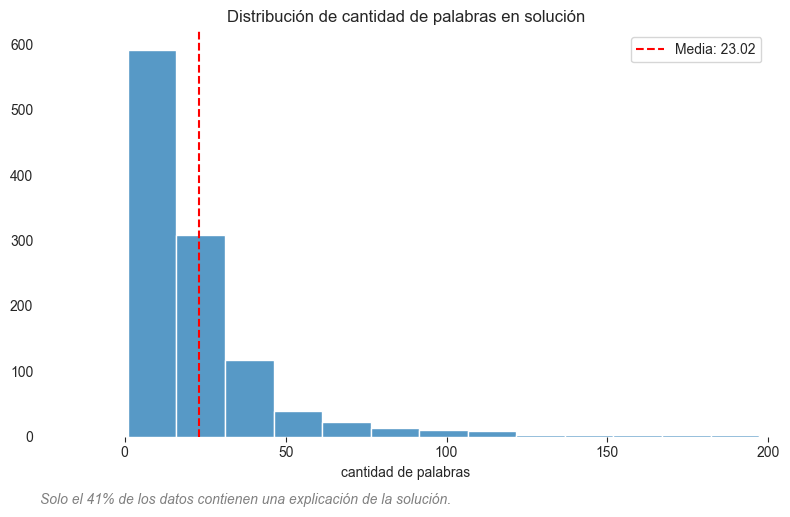
\includegraphics[width=0.85\linewidth]{cantidad de palabras solucion.png}
    \end{figure}
    {\small El análisis exploratorio reveló que menos de la mitad de los tickets traían
    solución escrita. Esto pesó en las decisiones que vinieron después.}
\end{frame}
\note{
IDEA CENTRAL: Esta imagen ES el argumento. El momento de la confirmación.

Tras extraer TODOS los datos que se pudieron, esta gráfica fue la prueba:
menos de la mitad tenían solución. Aquí se confirma lo que sospechábamos:
la base de conocimientos, tal como nos la describieron, NO existía.

Es el punto de giro del proyecto: deja de ser "consultar lo que hay" y se
transforma en "generar y atrapar el conocimiento que se está fugando".

IMAGEN: gráfica de cantidad de palabras en solución (la del 41%).
[Contesta: evidencia visual del POR QUÉ.]
}


% =====================================================================
%  ACTO 3 — LA DECISIÓN QUE CAMBIÓ EL RUMBO
% =====================================================================


\begin{frame}{Desbalance de clases}
    \begin{figure}\centering
        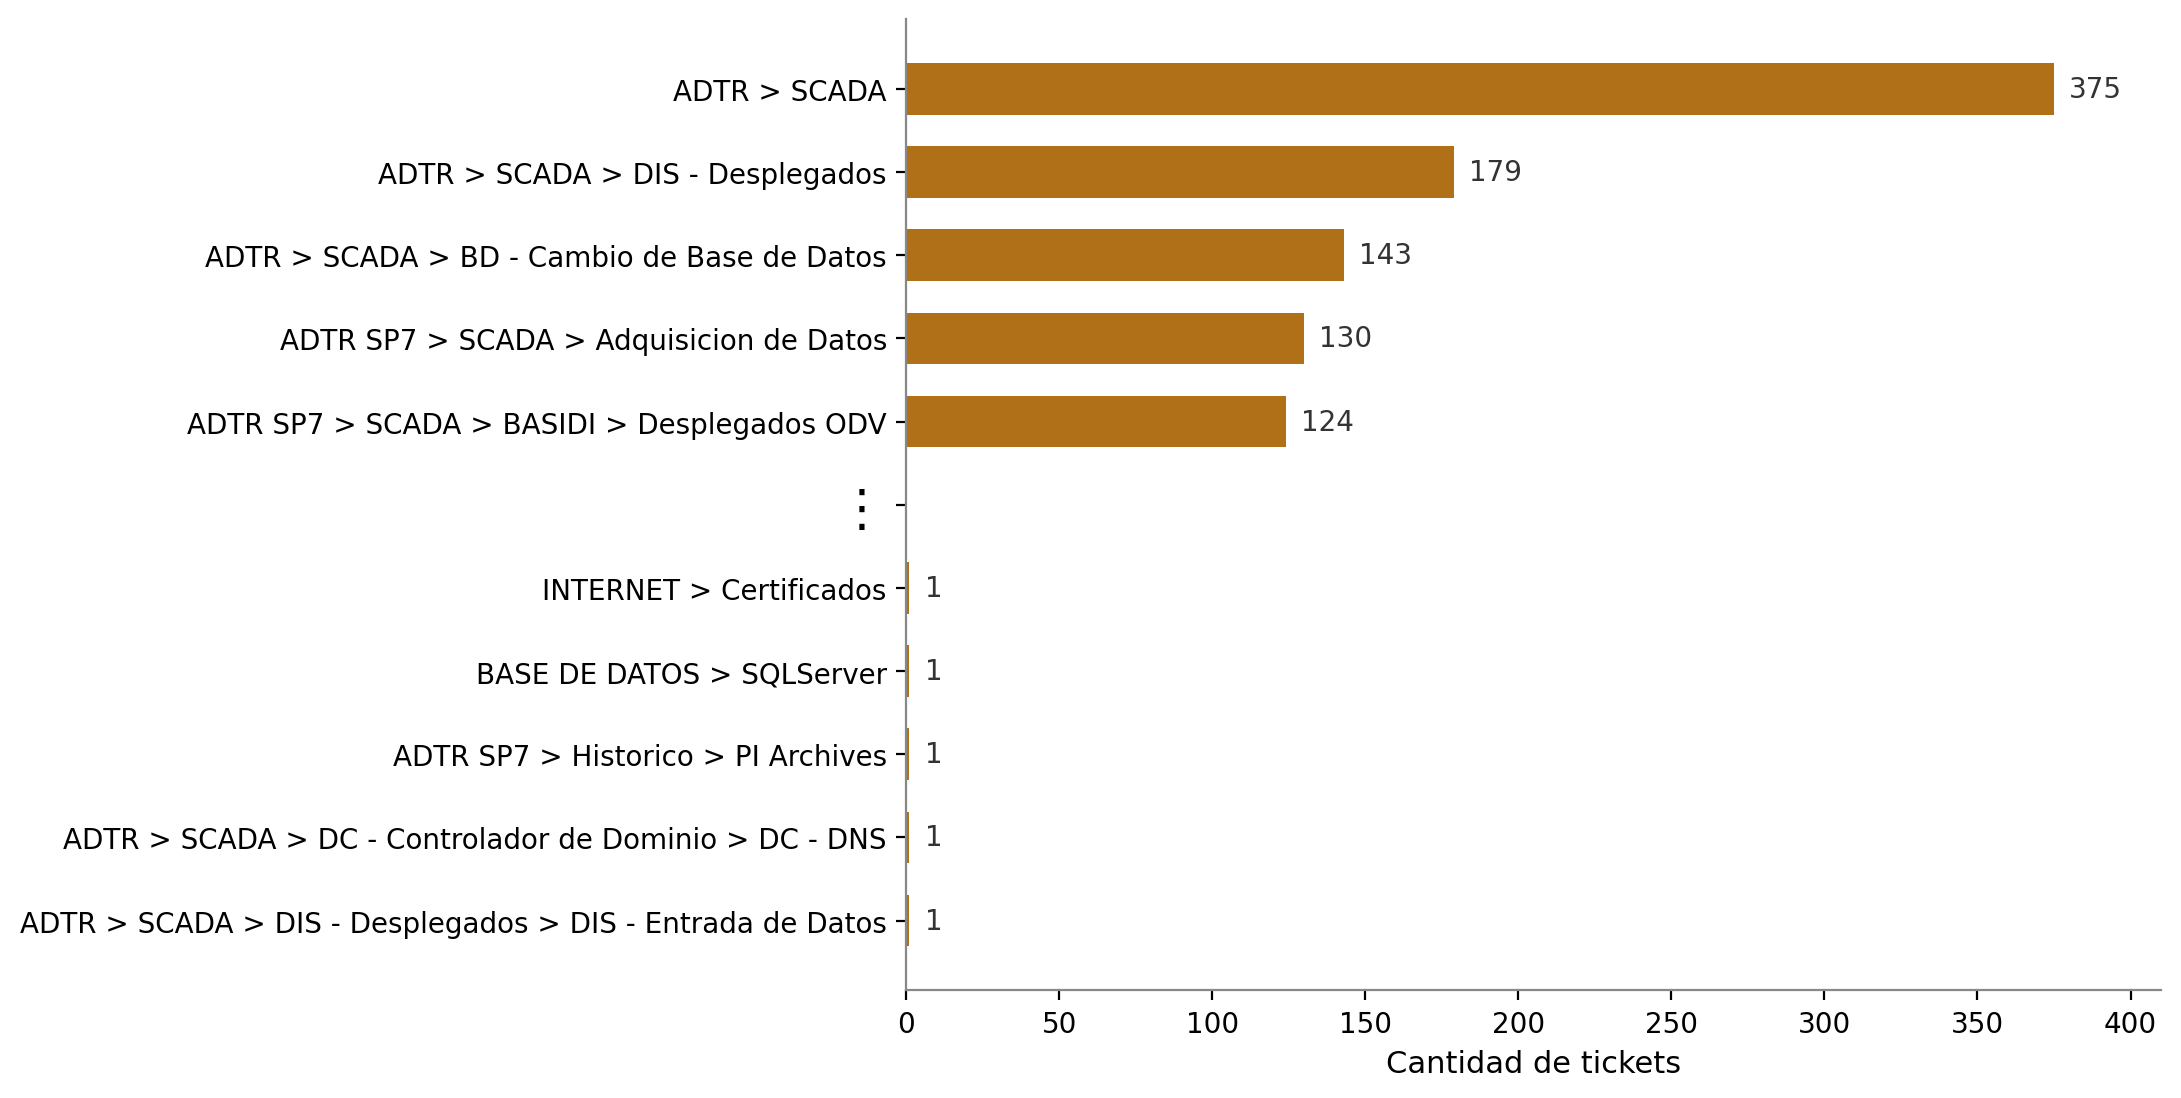
\includegraphics[width=1.0\linewidth]{desbalance_antes.png}
    \end{figure}
\end{frame}

\begin{frame}{Agrupación de categorías}
    \begin{figure}\centering
        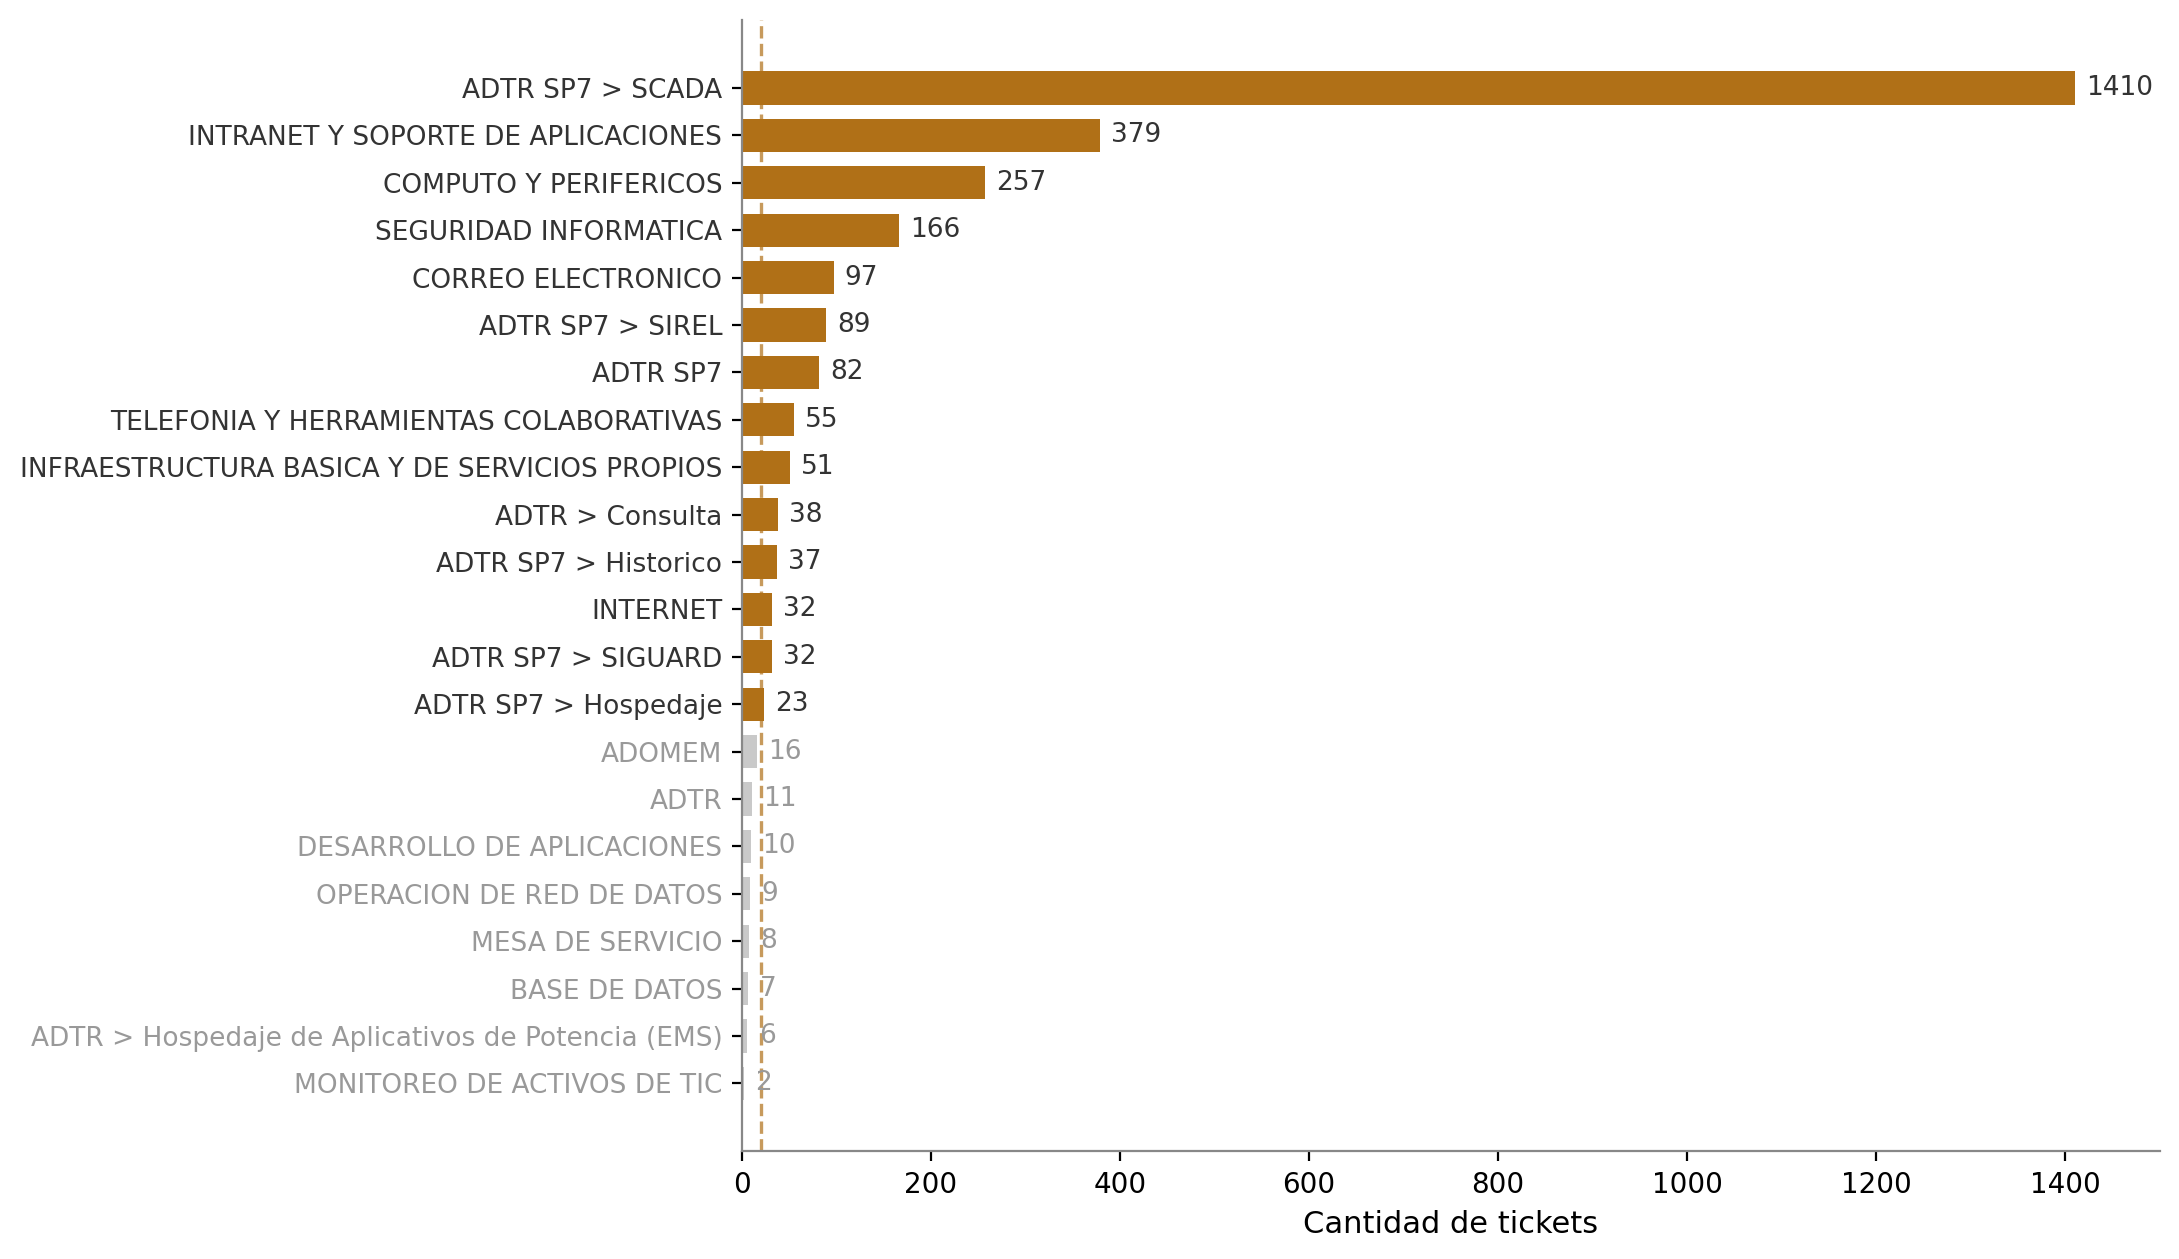
\includegraphics[width=0.92\linewidth]{desbalance_despues.png}
    \end{figure}
\end{frame}

% --- Lámina 10: Entrenamos los clasificadores ---
\begin{frame}{¿En qué categoría va este ticket?}
    Dos tickets fáciles de ubicar:
    \begin{itemize}
        \item «Reporte de falla en PC» $\rightarrow$ \textbf{Cómputo y periféricos}
        \item «Solicitud de bloqueo de dirección IP» $\rightarrow$ \textbf{Seguridad informática}
    \end{itemize}

    \bigskip
    ¿Y este?
    \begin{itemize}
        \item «Solicitud para instalar un visor de archivos .dwg (AutoCAD)»
        \quad \textcolor{orange!80!black}{\textbf{¿Cómputo o seguridad?}}
    \end{itemize}

    \vspace{0.4em}
    {\small Queríamos que la computadora hiciera esta misma elección, sola, con miles de tickets.}
\end{frame}
\note{
Gancho conceptual antes de los números: la clasificación es asignar a cada ticket su
categoría. Dos ejemplos caen claro; el tercero (instalar un visor de AutoCAD) cabe igual en
cómputo o en seguridad. Así el público entiende qué es clasificar y por qué es difícil,
antes de ver los F1. El detalle (con la etiqueta real) está en el apéndice.}

\begin{frame}{Modelos de clasificación}
    Entrenamos varios modelos para clasificar los tickets a partir de su texto.
    \begin{figure}
        \centering
        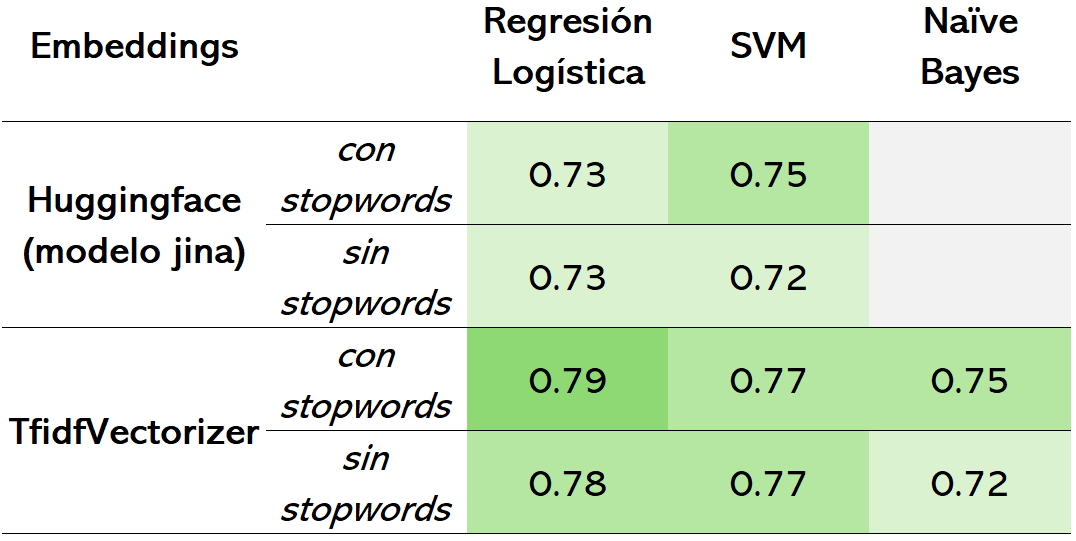
\includegraphics[width=0.82\linewidth]{matriz de resultados.png}
    \end{figure}
    {\small El F1-score va de 0 a 1 y resume qué tan bien se acierta la categoría cuando las
    clases están desbalanceadas. Con los primeros datos llegamos a 0.71 y con más datos a
    0.79. Unas categorías tenían cientos de tickets y otras casi ninguno, y eso
    marcó el límite.}
\end{frame}
\note{
IDEA CENTRAL: Dar el resultado honesto y explicar el porqué SIN jerga.

"Un modelo aprende de ejemplos, y es tan bueno como los ejemplos que le
das. Aun con 2,800 tickets, los datos no tenían la riqueza para enseñarle
a clasificar bien: unas categorías tenían cientos de casos y otras apenas
uno."

IMAGEN: tabla de resultados (matriz de resultados / F1-Score).
La matriz de confusión y la curva ROC van al APÉNDICE (no aquí).
[Contesta: CÓMO (resultado honesto).]
}

% --- Lámina 11: La decisión madura ---
\begin{frame}
    \begin{center}
        En acuerdo con el equipo del CENACE, decidimos \textbf{dejar el modelo de clasificación fuera del sistema final} y concentrar el esfuerzo en el \textbf{asistente}.
    \end{center}
\end{frame}
\note{
IDEA CENTRAL: Momento de FORTALEZA, no de disculpa.

Aquí es donde demuestro criterio de científico: cuando los datos no dan,
se ajusta el rumbo. El comité valora esto enormemente. Decirlo con la
cabeza en alto. Esta es la pata que "se cayó" del Acto 1, ahora explicada.
[Contesta: CÓMO (criterio científico).]
}

% =====================================================================
%  ACTO 4 — LA SOLUCIÓN: EL ASISTENTE QUE LEE POR TI
% =====================================================================

% --- Lámina 12: ¿Qué construimos? (en humano) ---
\begin{frame}{\textquestiondown Qué construimos?}
    \begin{center}
        \large
        Imaginen un asistente al que le entregamos \textbf{todos los manuales}
        del CENACE.

        \bigskip
        No los memoriza: \textbf{sabe dónde encontrarlos}.

        \bigskip
        Cuando un ingeniero pregunta algo, el asistente busca la información más relevante,
        arma una respuesta basada \textbf{solo con esa información}, y dice
        \textbf{de qué documento la sacó}.
    \end{center}
\end{frame}
\note{
IDEA CENTRAL: Explicar el RAG en lenguaje humano ANTES del diagrama.

Analogía (con moderación): el asistente bibliotecario. La clave que hay
que recalcar: "dice de dónde la sacó". Eso es lo que separa RESPONDER de
INVENTAR. Es la base de la confianza en un entorno técnico.
[Contesta: QUÉ (en lenguaje humano).]
}

\begin{frame}{Cómo funciona por dentro}
\begin{center}
\resizebox{\textwidth}{!}{%
\begin{tikzpicture}[
    font=\sffamily\small,
    >={Stealth[length=2.5mm]},
    caja/.style={
        draw=black, rounded corners=2pt, align=center,
        minimum height=1cm, minimum width=2.2cm, inner sep=5pt,
        fill=white, thick
    },
    clave/.style={
        draw=structure.fg, rounded corners=2pt, align=center,
        minimum height=1cm, minimum width=2.2cm, inner sep=5pt,
        fill=structure.fg!10, very thick, text=black
    },
    final/.style={
        draw=structure.fg, rounded corners=2pt, align=center,
        minimum height=1cm, minimum width=2cm, inner sep=5pt,
        fill=structure.fg, text=white, very thick, font=\sffamily\bfseries
    },
    flecha/.style={->, thick},
    etiqueta/.style={font=\sffamily\scriptsize\itshape, text=gray}
]

% ---------- PARTE 1 — INGESTA ----------
\node[caja] (docs)   {Documentos\\\scriptsize(Manuales, guías, normas...)};
\node[caja, right=1.8cm of docs] (frag) {Fragmentos\\de texto};
\node[clave, right=1.8cm of frag] (num1) {Se vuelven\\vectores};
\node[draw=structure.fg, cylinder, shape border rotate=90, aspect=0.3,
      fill=structure.fg!10, very thick, minimum height=1.4cm, minimum width=2.2cm,
      align=center, right=1.8cm of num1] (db1) {Base de\\datos};

\draw[flecha] (docs) -- node[etiqueta, above, align=center]{se divide\\el texto} (frag);
\draw[flecha] (frag) -- (num1);
\draw[flecha] (num1) -- node[etiqueta, above, align=center]{se guardan} (db1);

\begin{scope}[on background layer]
    \node[draw=structure.fg!40, rounded corners=4pt, dashed, thick,
          fit=(docs)(frag)(num1)(db1), inner sep=14pt] (p1box) {};
\end{scope}
\node[anchor=west, text=structure.fg, font=\sffamily\bfseries, fill=white, inner sep=2pt]
     at ([xshift=10pt]p1box.north west) {Parte 1 — Se prepara la información};

% ---------- PARTE 2 — CONSULTA ----------
\node[caja, below=3.0cm of docs] (preg) {Pregunta\\del usuario};
\node[clave, right=1.8cm of preg] (num2) {Se vuelve\\vector};
\node[draw=structure.fg, cylinder, shape border rotate=90, aspect=0.3,
      fill=structure.fg!10, very thick, minimum height=1.4cm, minimum width=2.2cm,
      align=center, right=1.8cm of num2] (db2) {Base de\\datos};
\node[clave, right=1.8cm of db2] (rel) {Fragmentos\\relevantes};
\node[caja, below=1.4cm of rel] (mll) {Modelo de\\lenguaje};
\node[final, below=1.4cm of num2] (resp) {Respuesta};

\draw[flecha] (preg) -- (num2);
\draw[flecha] (num2) -- node[etiqueta, above, align=center]{se busca} (db2);
\draw[flecha] (db2) -- node[etiqueta, above, align=center]{lo más\\parecido} (rel);
\draw[flecha] (rel.south) -- (mll.north);
\draw[flecha] (mll) -- node[etiqueta, above]{redacta} (resp);
\draw[flecha] (preg.south) |- ([yshift=-0.86cm]preg.south) -| (mll.north)
      node[etiqueta, pos=0.25, above, align=center]{la pregunta también\\se entrega al modelo};

\begin{scope}[on background layer]
    \node[draw=structure.fg!40, rounded corners=4pt, dashed, thick,
          fit=(preg)(num2)(db2)(rel)(mll)(resp), inner sep=14pt] (p2box) {};
\end{scope}
\node[anchor=west, text=structure.fg, font=\sffamily\bfseries, fill=white, inner sep=2pt]
     at ([xshift=10pt]p2box.north west) {Parte 2 — Se responde una consulta};

\end{tikzpicture}%
}
\end{center}
\end{frame}

% =====================================================================
%  OPCIONAL — Revelar el diagrama en DOS láminas (primero la ingesta,
%  luego la consulta). Si lo prefieres así, usa DOS frames separados:
%  uno que contenga solo el bloque "PARTE 1" y otro con "PARTE 1 + PARTE 2".
%  Pídemelo y te dejo esa variante con \pause / \onslide ya armada.
% =====================================================================



% --- Lámina 14: El camino no fue recto (tropiezos técnicos condensados) ---
\begin{frame}
Probamos varias herramientas y modelos. Algunas simplemente
\textbf{no funcionaron como esperábamos}.

\bigskip
Hubo un reto \textbf{de los datos} que atacamos y resolvimos durante el trabajo:
\begin{itemize}
    \item[$\bullet$] Incidentes \textbf{truncados}: una extracción defectuosa cortó
    las descripciones y las soluciones a media frase. Obtuvimos el conjunto de datos
    completo y el problema quedó resuelto.
\end{itemize}

\bigskip
Y hay retos \textbf{del entorno} del CENACE con los que se opera a diario:
\begin{itemize}
    \item[$\bullet$] Tickets con \textbf{jerga técnica del dominio} y \textbf{errores ortográficos}.
    \item[$\bullet$] \textbf{Cómputo limitado} por trabajar on-premise.
\end{itemize}
\bigskip
Por eso ajustamos y reemplazamos componentes hasta dar con unos que entendieran este entorno.

\end{frame}

\note{
IDEA CENTRAL: Condensar TODOS los tropiezos técnicos en una sola idea.

No detallar los cinco cambios (Jina -> bge-m3, Phi4 -> gemma3, etc.). Para
esta audiencia, la idea es: "modelos entrenados con español formal vs.
nuestros tickets reales, informales y con errores".

Si el comité pregunta detalle técnico, lo tengo en reserva:
- Jina (768 dim) saturaba el espacio vectorial y venía de corpus formales
  (CulturaX, Wikipedia) -> domain shift.
- bge-m3: 1024 dim, multilingüe, ventana 8192. Mejor para nuestro caso.
- Modelo de lenguaje: cambio de Phi4 a gemma3:12b por ventana de contexto.
[Contesta: CON QUÉ MEDIOS (y el criterio para elegirlos).]
}

\begin{frame}{Persistencia}
    \begin{center}
        \large
        Cuando el asistente da una solución y el ingeniero la marca como
        \textbf{útil}, esa solución \textbf{se guarda} y se vuelve parte de la base de conocimientos.

        \bigskip
        La próxima vez que alguien tenga un problema parecido, \textbf{esa
        solución ya está ahí}.
    \end{center}

    \bigskip
    \begin{center}
        \textbf{El conocimiento que antes se iba, ahora se queda y crece.}
    \end{center}
\end{frame}
\note{
IDEA CENTRAL: ESTE es el momento memorable. Bajar el ritmo. Dar aire.

Recordar al enemigo del Acto 1 y cerrarlo:
"Al inicio les dije que el conocimiento se perdía. Aquí está la respuesta."

Frase de clímax (decirla despacio, con pausa):
"El sistema no solo responde: aprende de cada solución que funciona. El
conocimiento que antes se evaporaba, ahora se queda y crece."

Si la audiencia se lleva UNA sola cosa, que sea esta.
[Contesta: el cierre del POR QUÉ. El momento memorable.]
}

% --- Lámina 15: El prototipo, funcionando (capturas) ---
\begin{frame}{Prototipo final}
    \begin{figure}
        \centering
        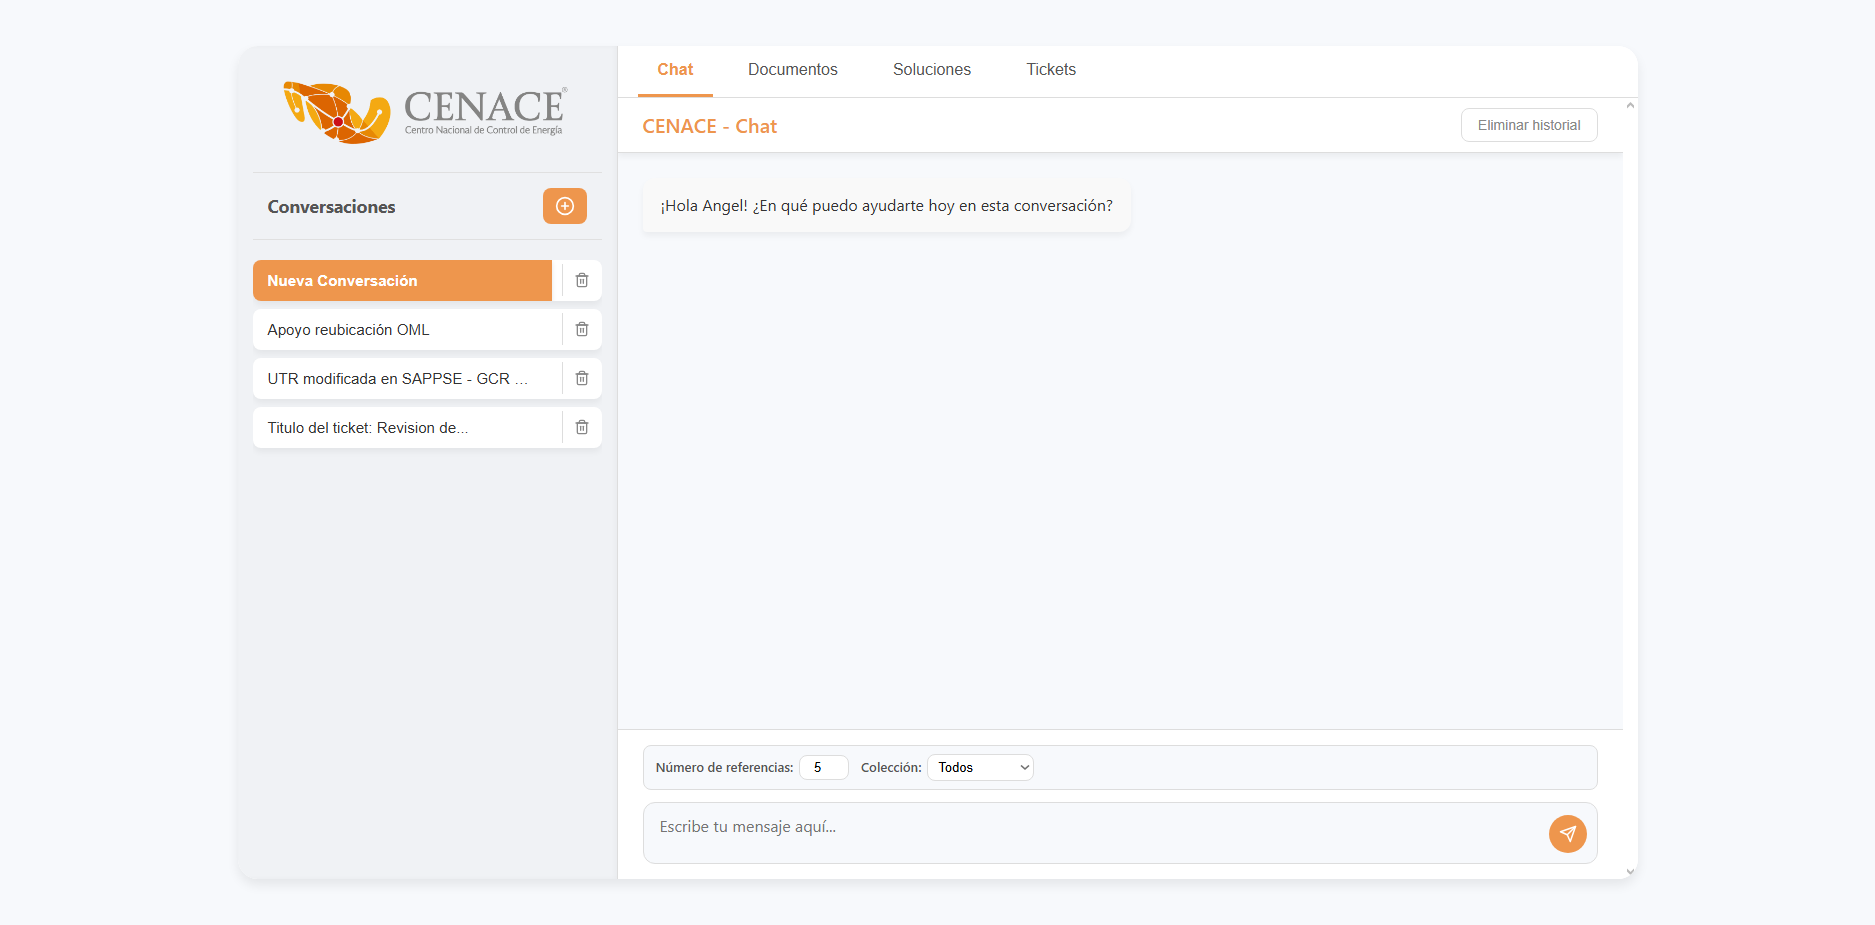
\includegraphics[width=1.0\linewidth]{sesion_chat.png}
    \end{figure}
\end{frame}
\note{
IDEA CENTRAL: Mostrar lo TANGIBLE. A la audiencia le encanta ver la cosa
real funcionando.

Pasar por las pestañas (Chat, Documentos, Soluciones, Tickets) con ritmo
ágil para mostrar que existe y corre. Las siguientes láminas son esas
pestañas. No detenerse demasiado en cada una.

IMAGEN: sesion_chat.png (y las siguientes pestañas).
[Contesta: QUÉ (la prueba palpable).]
}

% --- Láminas 15b-15e: recorrido de pestañas del prototipo (rápido) ---
\begin{frame}{Prototipo final}
    \begin{figure}
        \centering
        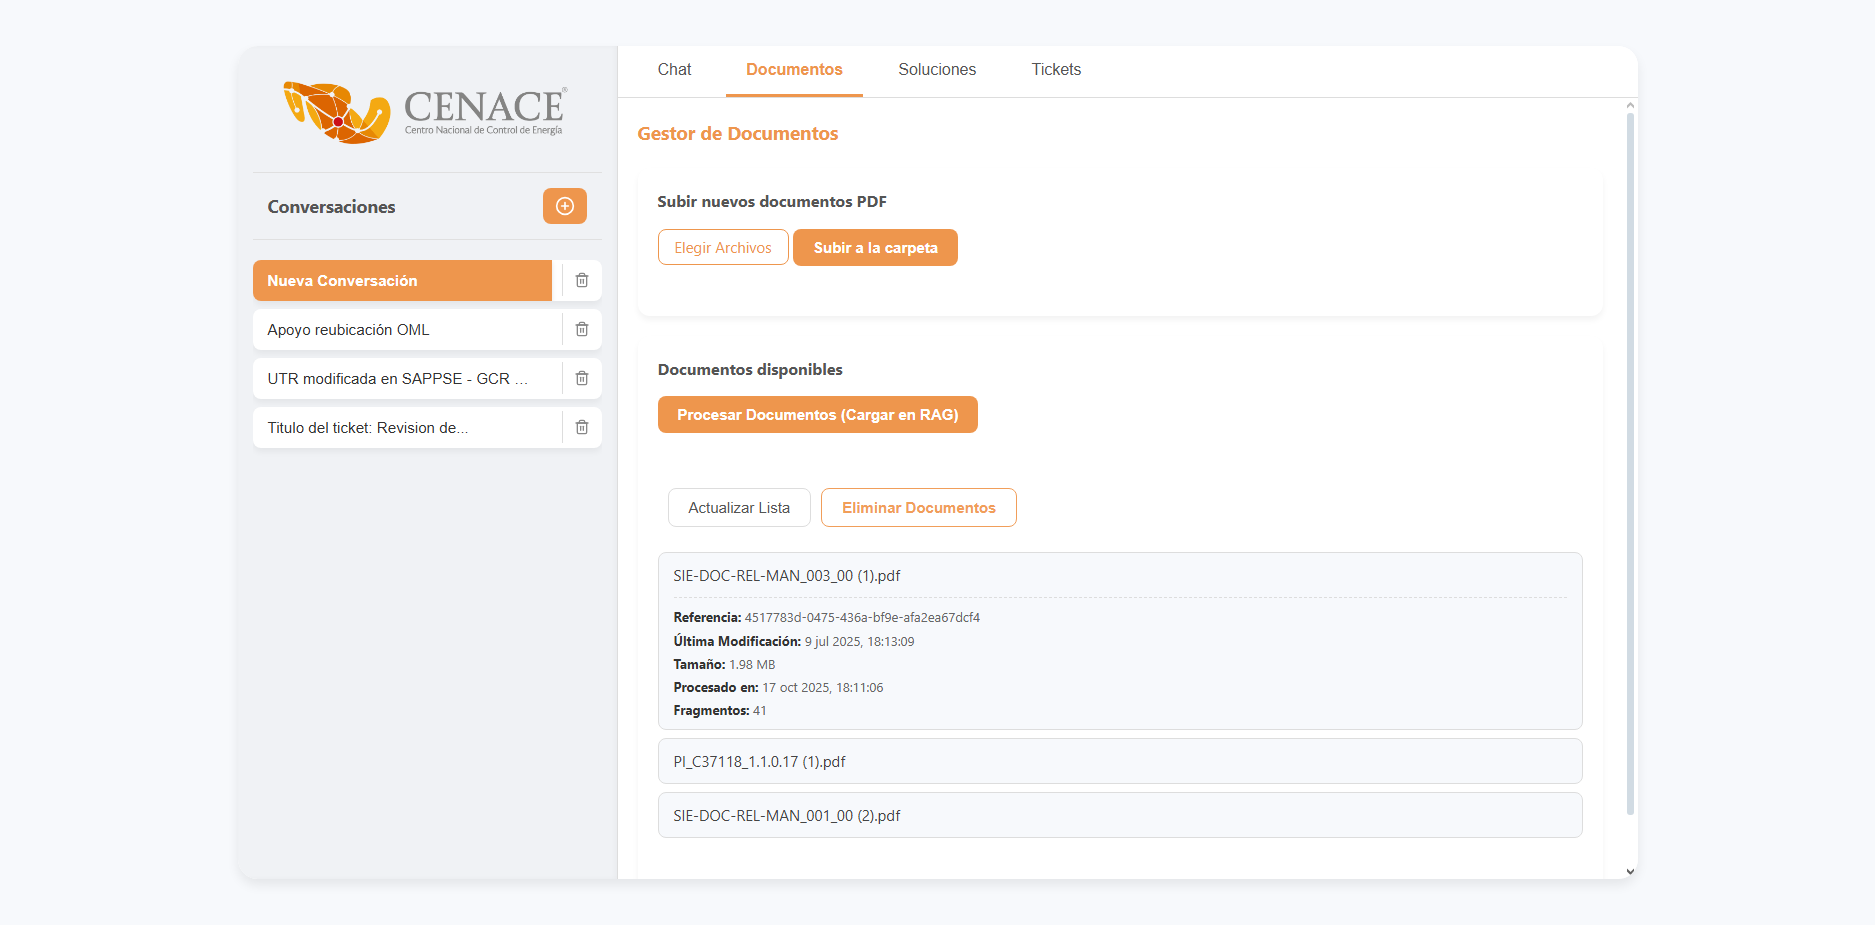
\includegraphics[width=1.0\linewidth]{sesion_documentos.png}
    \end{figure}
\end{frame}
\note{
IDEA CENTRAL: Aquí el usuario CARGA documentos PDF a la base.
Pasar rápido. Mostrar que se puede nutrir el sistema con nueva
documentación.
}

\begin{frame}{Prototipo final}
    \begin{figure}
        \centering
        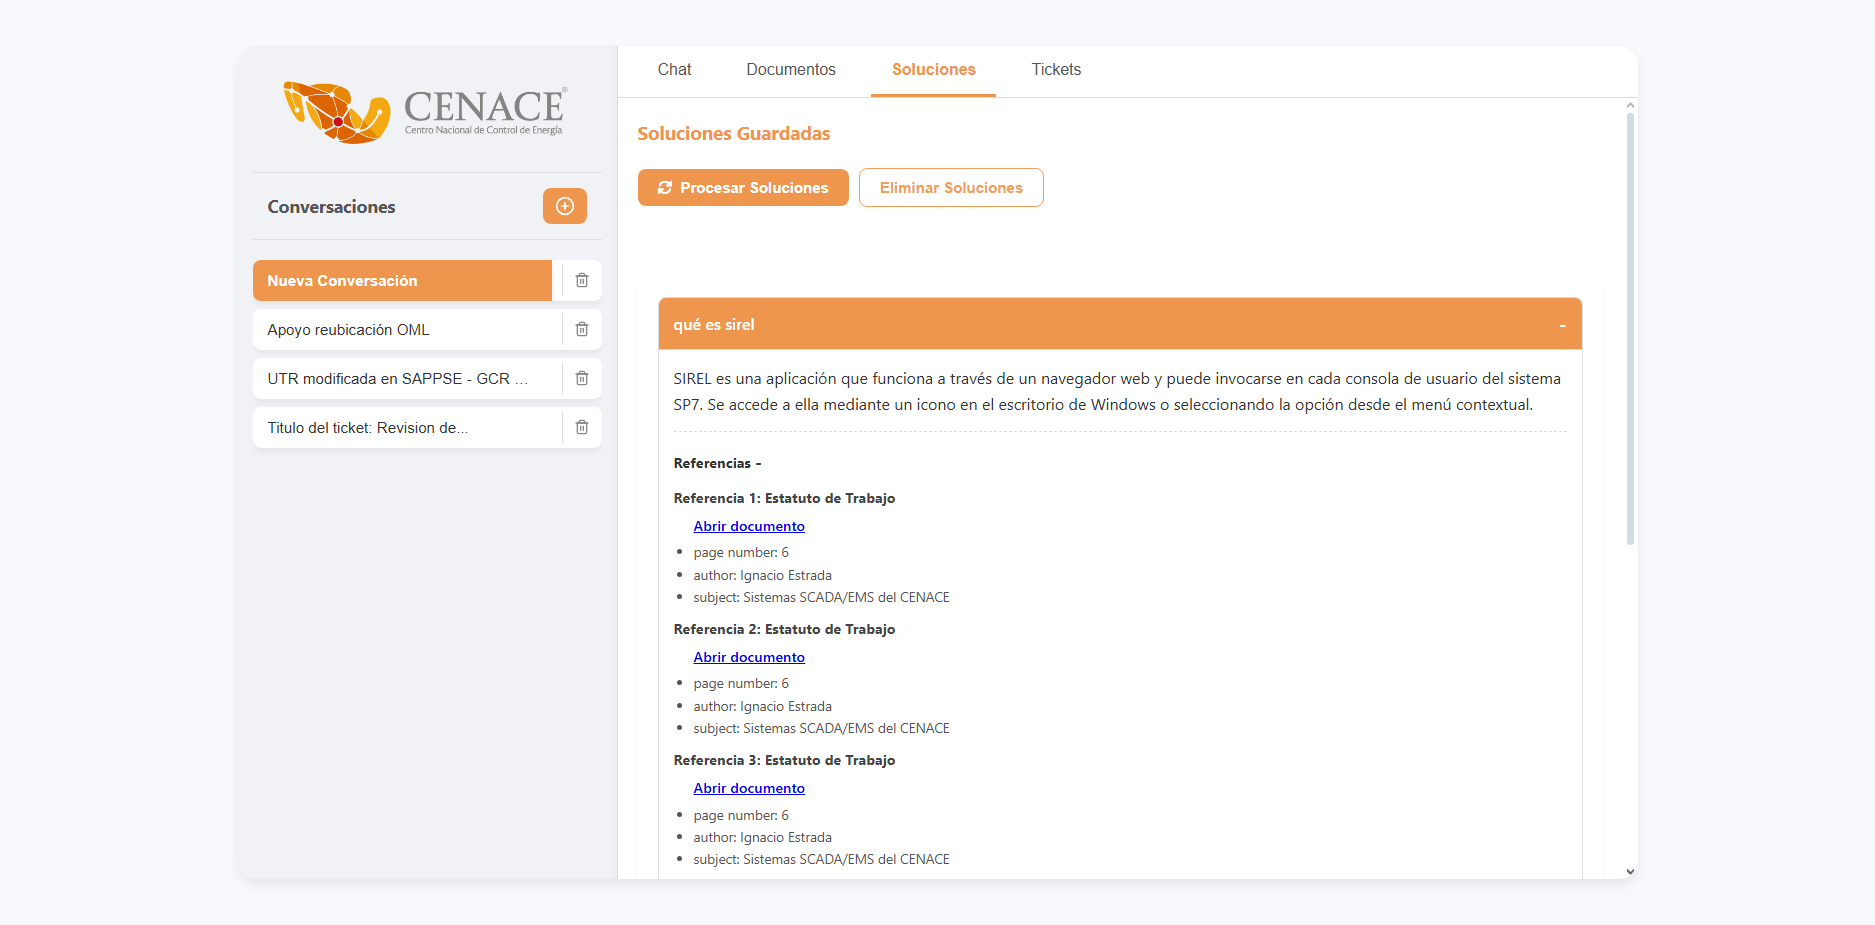
\includegraphics[width=1.0\linewidth]{sesion_soluciones.png}
    \end{figure}
\end{frame}
\note{
IDEA CENTRAL: Esta pestaña es la ANTESALA del clímax.
Aquí viven las soluciones marcadas como útiles, con sus referencias.
Sembrar: "fíjense que cada solución guarda de dónde salió". Esto conecta
directo con la lámina del ciclo. Pasar con intención, no de prisa.
}

\begin{frame}{Prototipo final}
    \begin{figure}
        \centering
        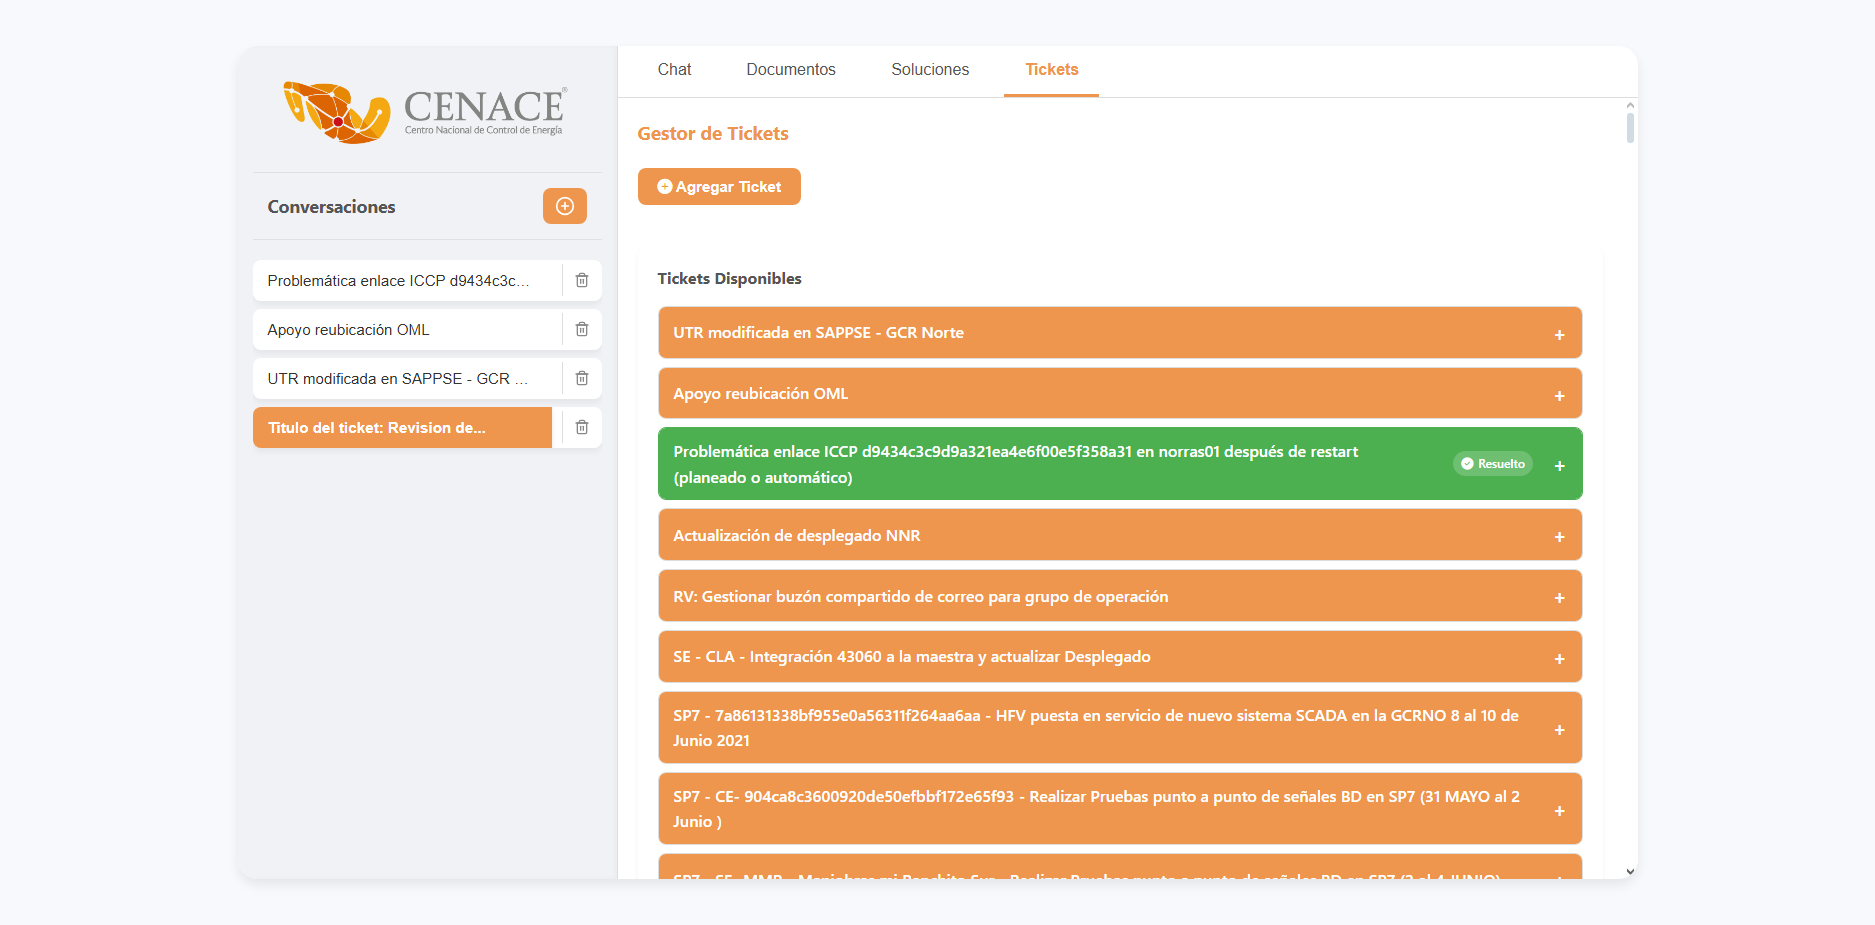
\includegraphics[width=1.0\linewidth]{sesion_tickets.png}
    \end{figure}
\end{frame}
\note{
IDEA CENTRAL: Los tickets se pueden mandar a una conversación con el
asistente para iterar hacia la solución. Pasar rápido.
}




% --- Lámina 19: Cierre ---
\begin{frame}{Futuro}
    \begin{center}
        \large
        Cada solución que los ingenieros validan hace crecer un corpus que
        algún día permitirá entrenar \textbf{modelos propios del CENACE}.

        \bigskip
        El sistema es capaz de adaptarse y pasar de ser el centro del flujo, a convertirse en un herramienta para un agente.
    \end{center}
\end{frame}
\note{
IDEA CENTRAL: Reposo. Cerrar el hilo rojo. Volver a la semilla.

Conectar el ciclo con el futuro: el conocimiento que se atrapa hoy es la
materia prima para modelos propios mañana. Terminar con calma, agradecer,
y abrir preguntas.
[Contesta: cierra el hilo rojo. Reposo.]
}

% =====================================================================
%  APÉNDICE — Material de respaldo para preguntas del comité
%  (Estas láminas NO se presentan; se usan solo si preguntan.)
% =====================================================================

\begin{frame}{Apéndice: Cronograma de actividades}
\begin{table}
    \centering
    \resizebox{\textwidth}{!}{%
    \begin{tabular}{|c|l|c|c|}
    \hline
    \textbf{Fase} & \textbf{Actividad} & \textbf{Fecha de Inicio} & \textbf{Fecha de Finalización} \\ \hline
    Fase 1 & Tratamiento de los datos & 04/05/2024 & 09/07/2024
    \\ \hline
    Fase 2 & Entrenamiento del modelo de clasificación & 19/05/2024 & 27/06/2024 \\ \hline
    Fase 3 & Implementación de la base de conocimientos & 01/10/2024 & 05/01/2025
    \\ \hline
    Fase 4 & Conexión de sistemas & 10/01/2025 & 10/03/2025
    \\ \hline
    Fase 5 & Desarrollo del prototipo final del chatbot & 12/03/2025 & 12/05/2025
    \\ \hline
    \end{tabular}%
    }
    \caption{Cronograma de Actividades del Proyecto}
    \label{tab:cronograma}
\end{table}
\end{frame}
\note{
APÉNDICE: Mostrar solo si preguntan por tiempos/fechas.
}

\begin{frame}{Apéndice: EDA — palabras en título}
    \begin{figure}\centering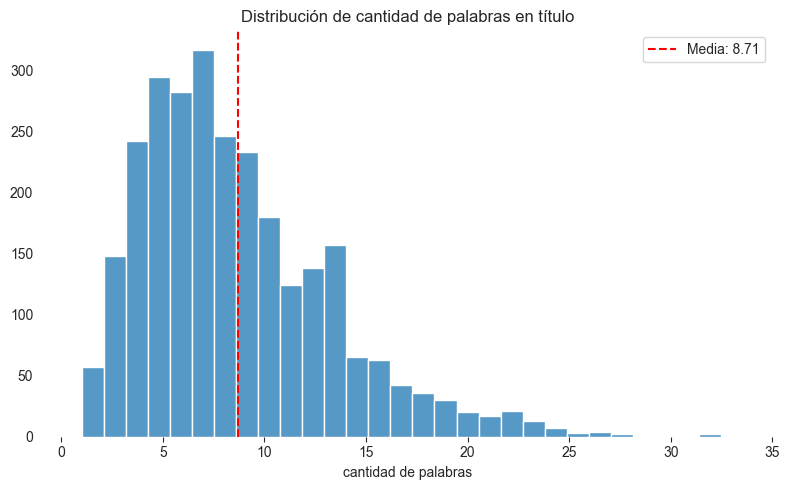
\includegraphics[width=1.0\linewidth]{cantidad de palabras titulo.png}\end{figure}
\end{frame}
\note{APÉNDICE: respaldo del EDA.}

\begin{frame}{Apéndice: EDA — palabras en descripción}
    \begin{figure}\centering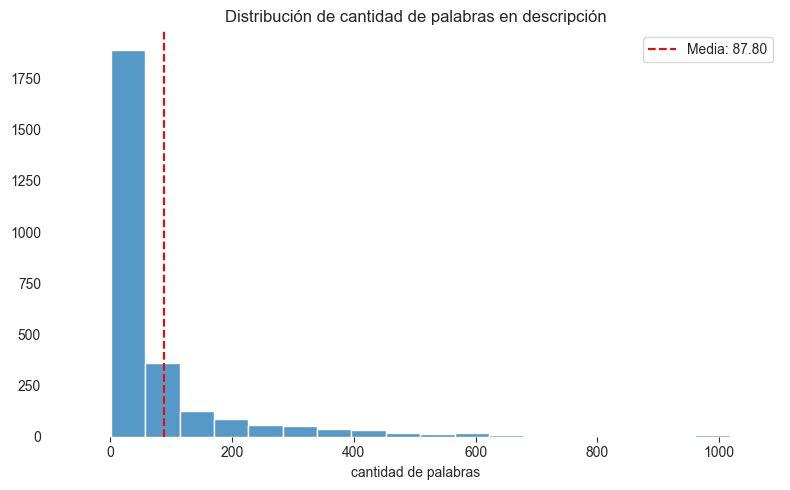
\includegraphics[width=1.0\linewidth]{cantidad de palabras descripcion.png}\end{figure}
\end{frame}
\note{APÉNDICE: respaldo del EDA. Aquí se nota el truncamiento de descripciones.}

\begin{frame}{Apéndice: Bigramas en título}
    \begin{figure}\centering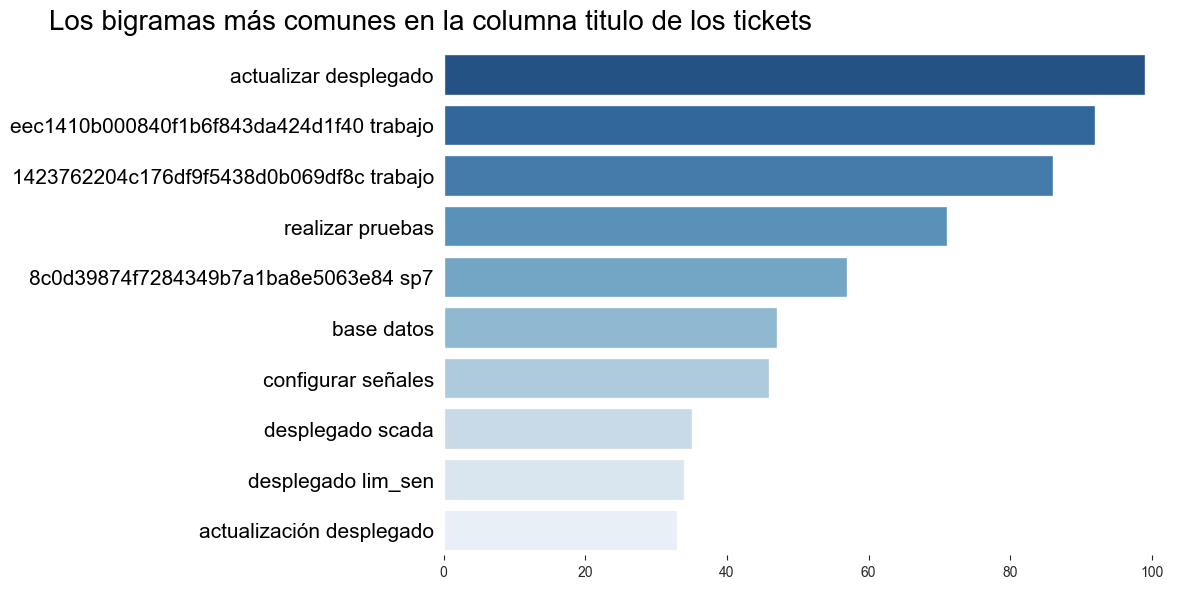
\includegraphics[width=1.0\linewidth]{bigrama titulo.png}\end{figure}
\end{frame}
\note{APÉNDICE: respaldo del EDA.}

\begin{frame}{Apéndice: Bigramas en descripción}
    \begin{figure}\centering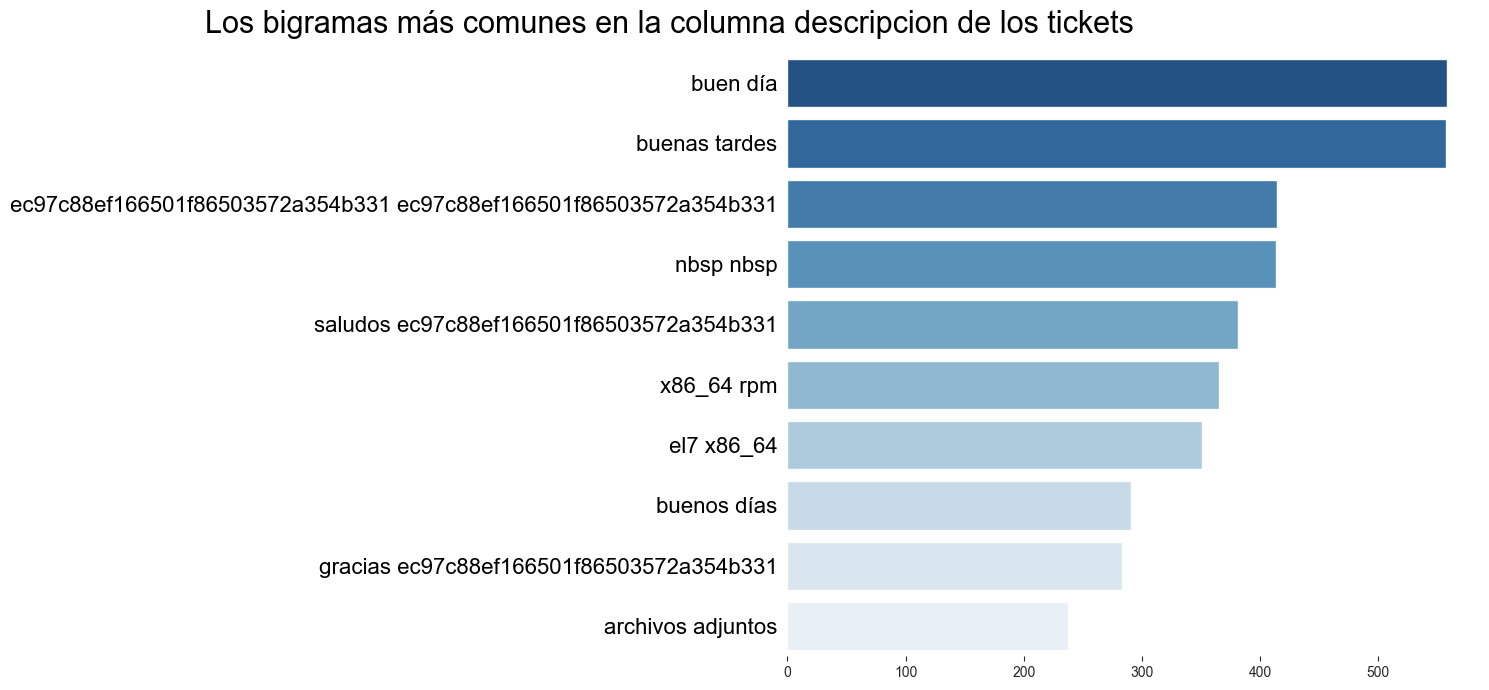
\includegraphics[width=1.0\linewidth]{bigrama descripcion.png}\end{figure}
\end{frame}
\note{APÉNDICE: respaldo del EDA.}

\begin{frame}{Apéndice: Bigramas en solución}
    \begin{figure}\centering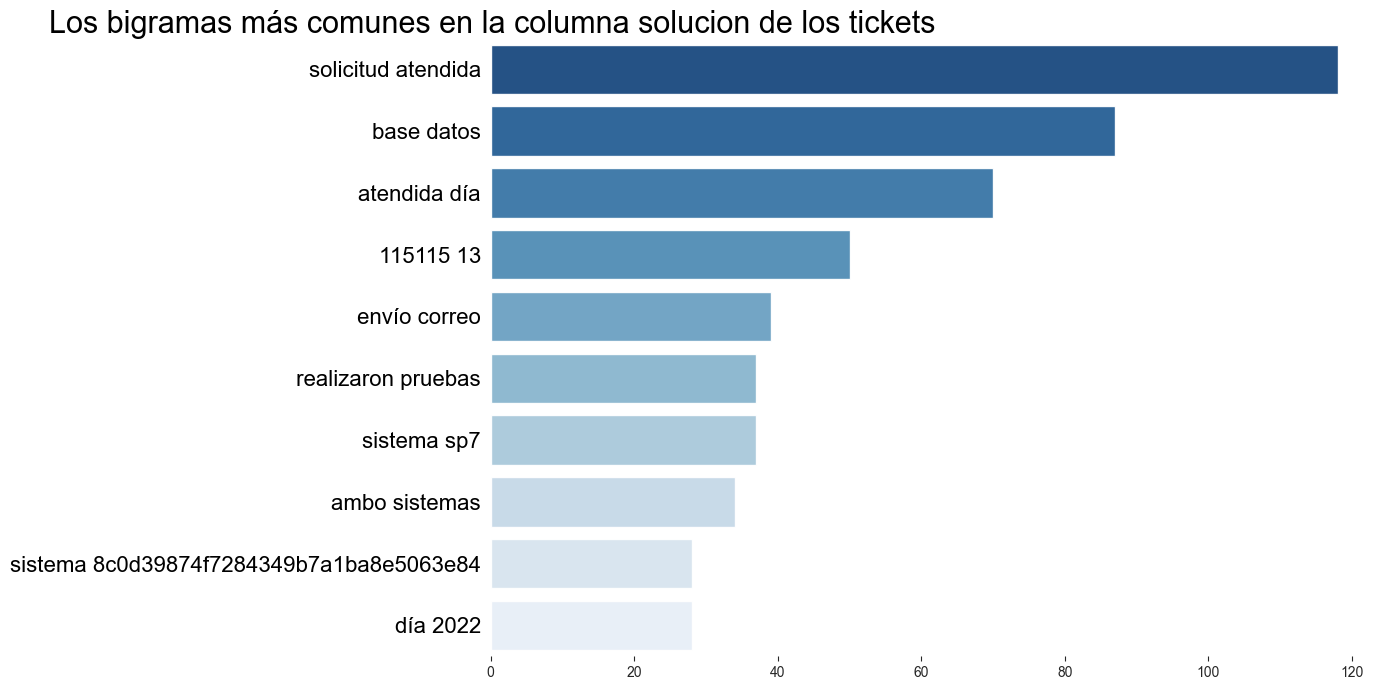
\includegraphics[width=1.0\linewidth]{bigrama solucion.png}\end{figure}
\end{frame}
\note{APÉNDICE: respaldo del EDA.}

\begin{frame}{Apéndice: Nube de palabras (solución)}
    \begin{figure}\centering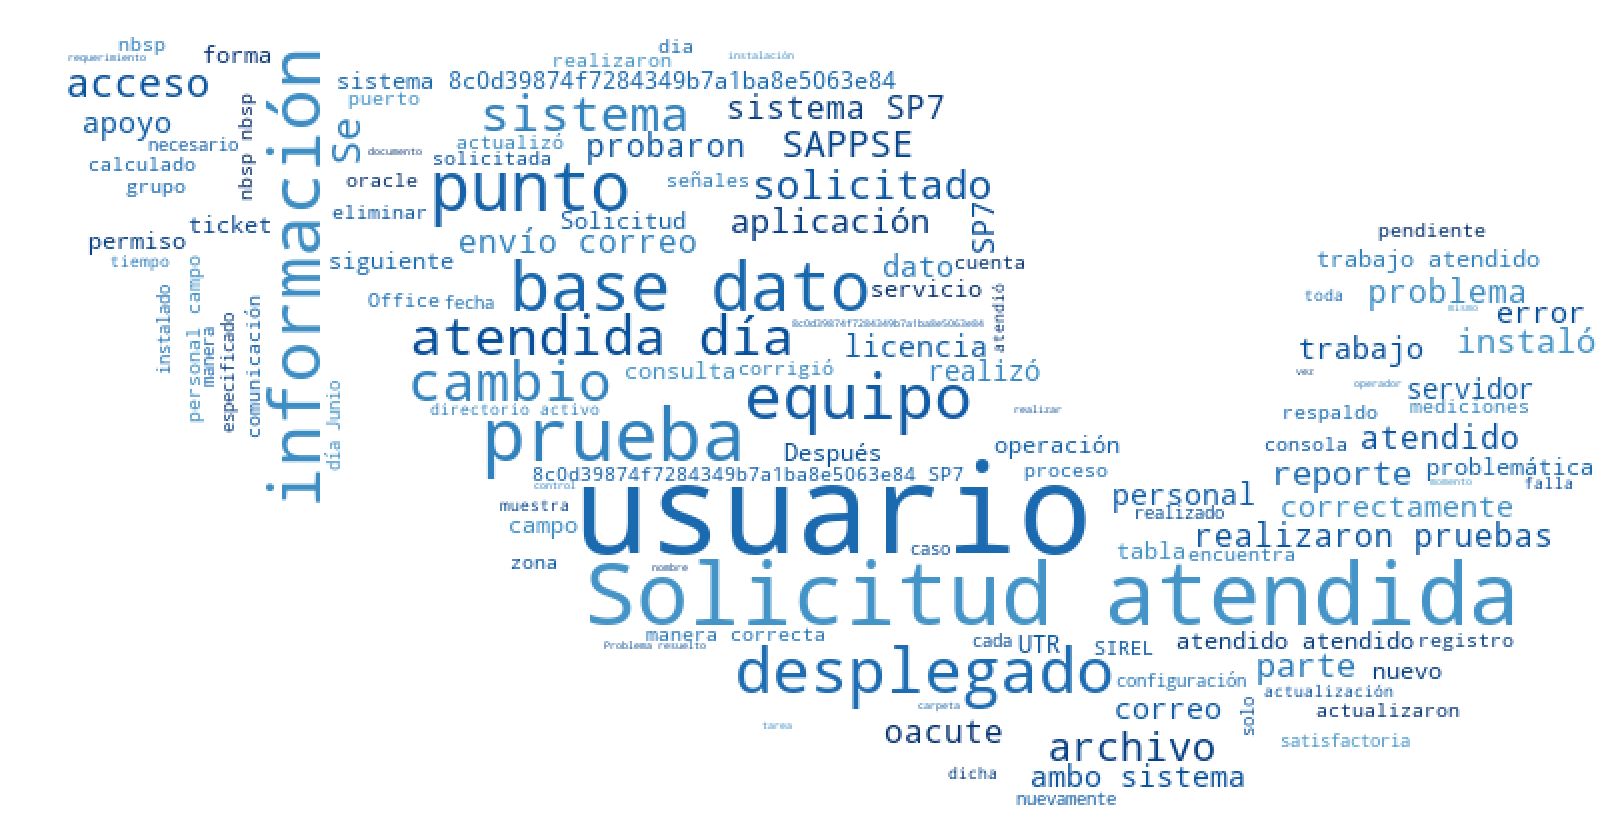
\includegraphics[width=1.0\linewidth]{wordcloud solucion.png}\end{figure}
\end{frame}
\note{APÉNDICE: respaldo del EDA.}

\begin{frame}{Apéndice: Matriz de confusión (Regresión Logística)}
    \begin{figure}\centering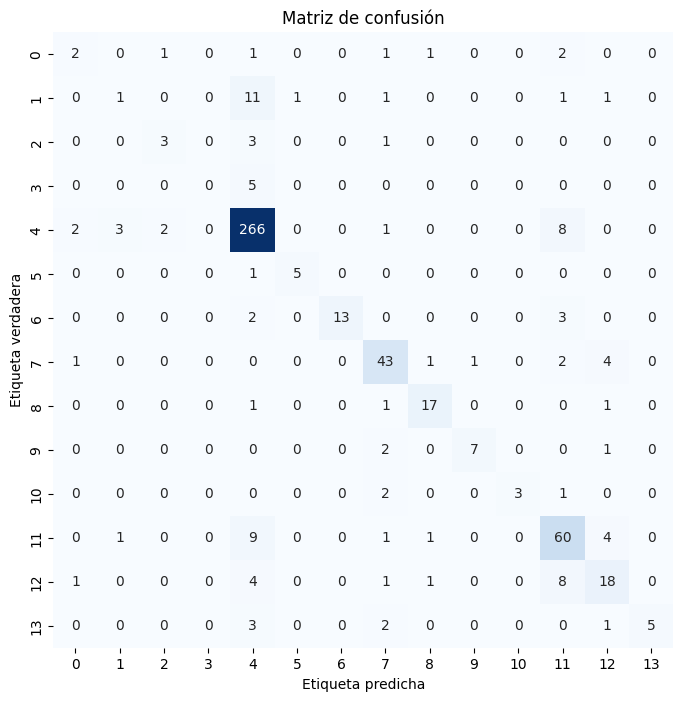
\includegraphics[width=0.65\linewidth]{matriz de confusion LR.png}\end{figure}
\end{frame}
\note{
APÉNDICE: mostrar si preguntan por detalle del clasificador.
La diagonal concentra los aciertos; la clase mayoritaria (ADTR > SCADA)
domina; las clases minoritarias dispersan errores -> poco dato.
}

\begin{frame}{Apéndice: Curvas ROC multiclase}
    \begin{figure}\centering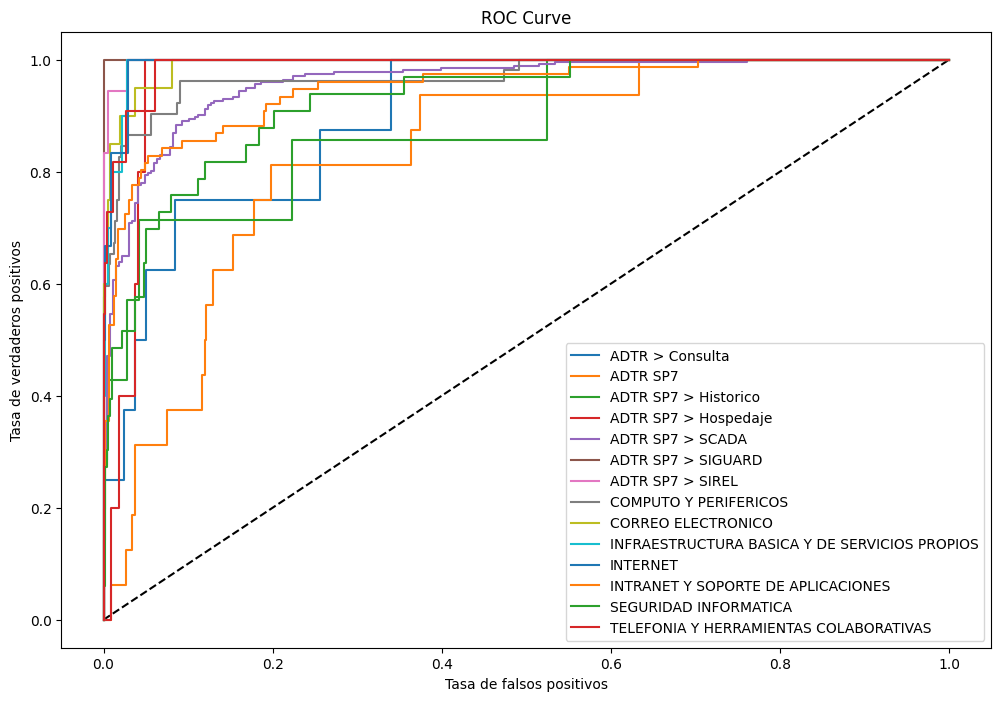
\includegraphics[width=0.95\linewidth]{curva roc.png}\end{figure}
\end{frame}
\note{
APÉNDICE: mostrar si preguntan por detalle del clasificador.
Curvas "a pasos" en clases con pocas muestras -> sensibles al umbral.
}

\begin{frame}{Apéndice: Desafíos}
    \begin{itemize}
        \item[$\bullet$] Los \textbf{errores ortográficos} dificultaron la identificación de patrones.
        \item[$\bullet$] Limitaciones en el \textbf{poder computacional disponible}.
        \item[$\bullet$] Los primeros conjuntos de datos estaban \textbf{truncados}.
    \end{itemize}
\end{frame}
\note{APÉNDICE: resumen de desafíos, por si surge la pregunta.}


% --- Lámina 13: Cómo funciona por dentro (diagrama RAG) ---
\begin{frame}{Apéndice: Sistema RAG}
   \begin{figure}
       \centering
        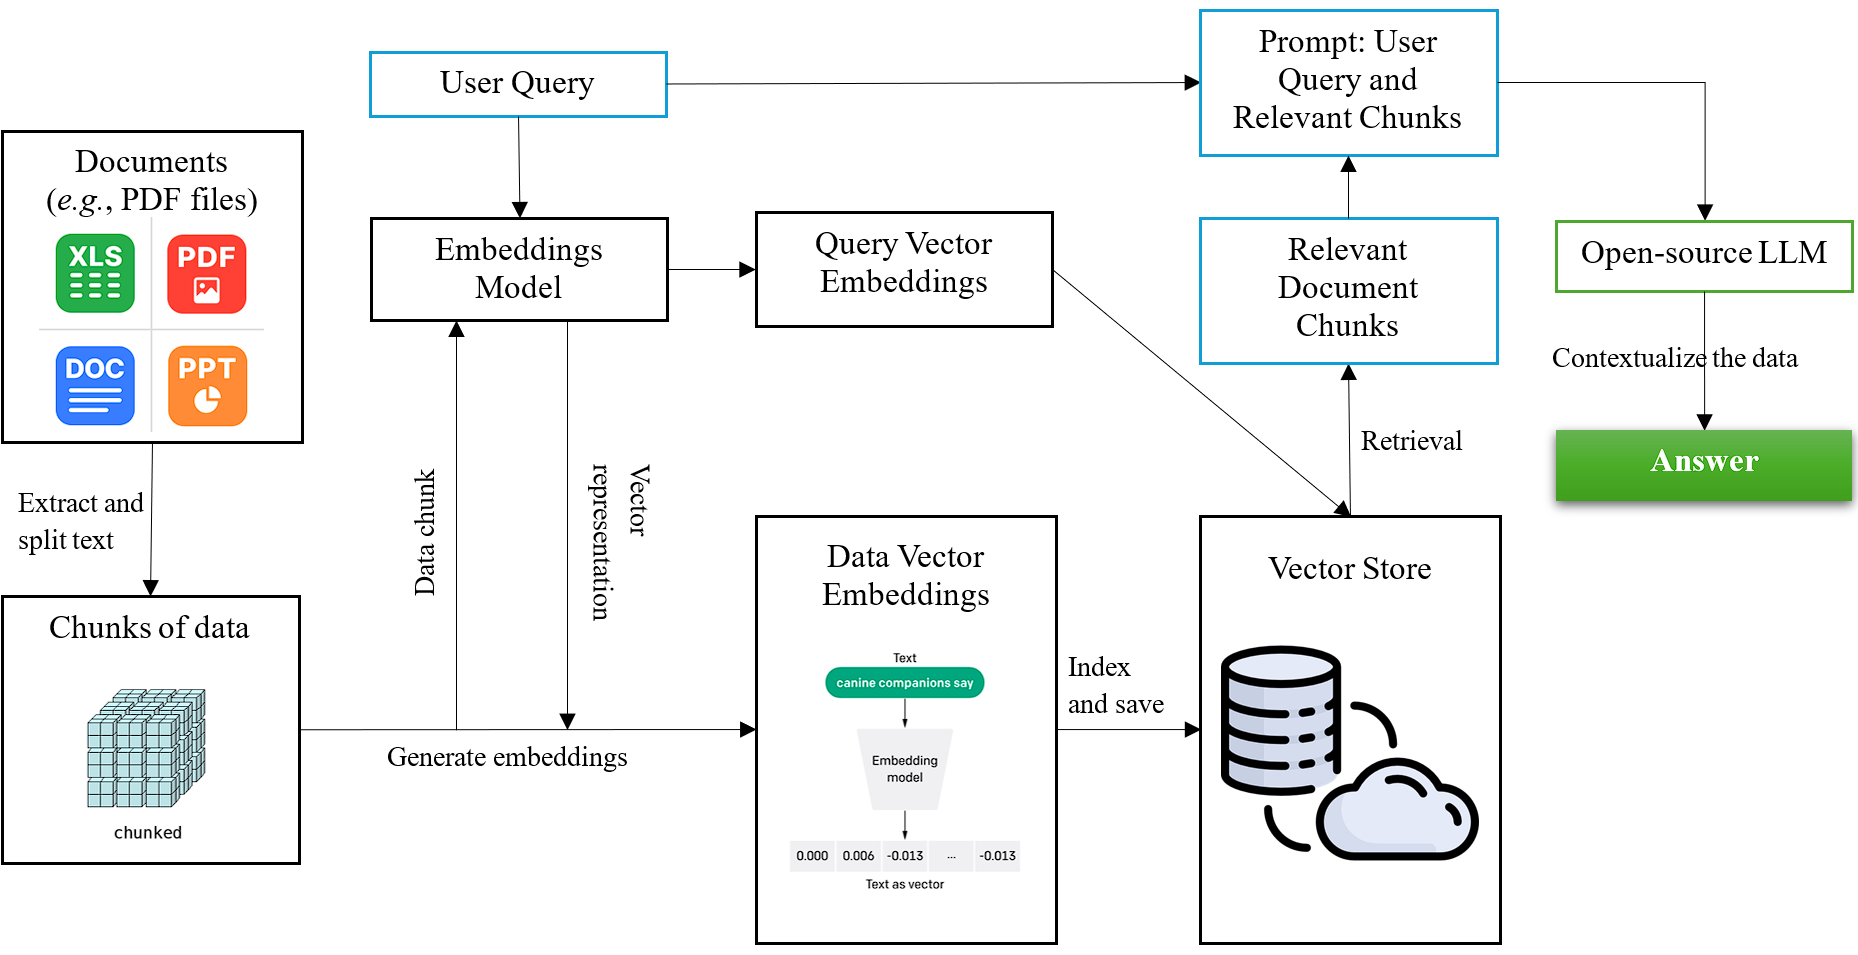
\includegraphics[width=1.0\linewidth]{image.png}
   \end{figure}
\end{frame}


\begin{frame}{Apéndice: Prototipo — inicio de sesión}
    \begin{figure}\centering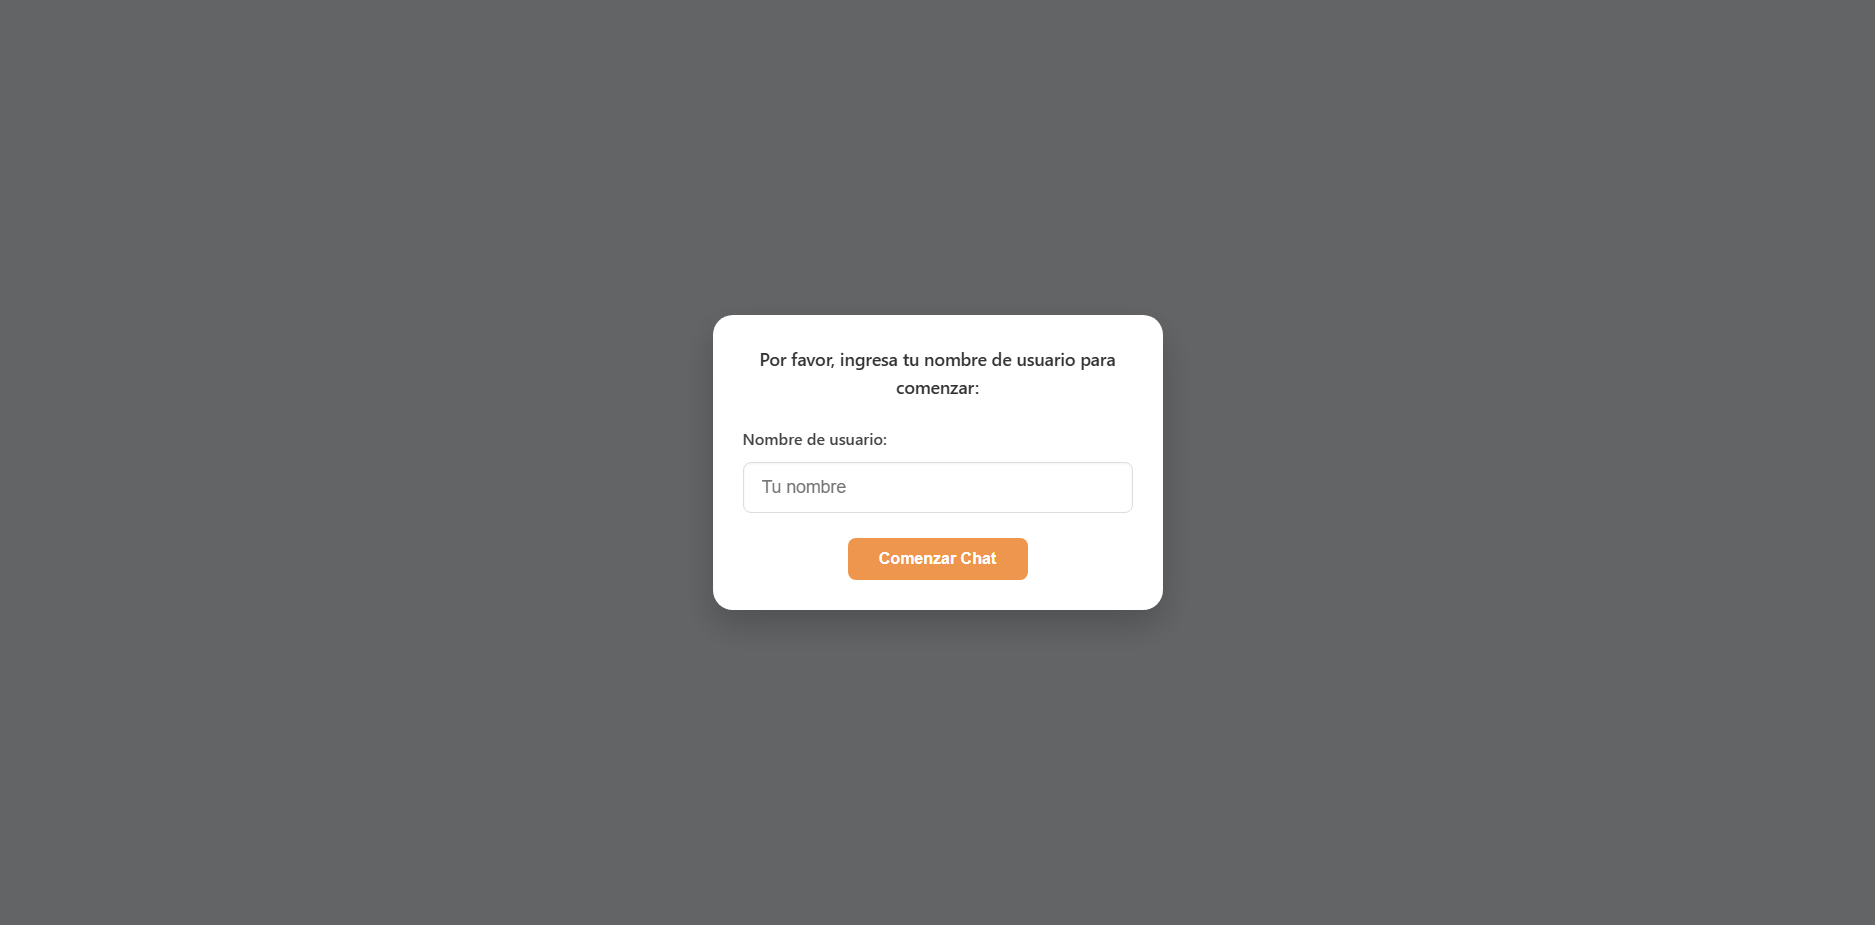
\includegraphics[width=1.0\linewidth]{sesion_inicio.png}\end{figure}
\end{frame}
\note{APÉNDICE: pantalla de inicio del prototipo.}

\begin{frame}{Apéndice: Prototipo (sketch inicial)}
    \begin{figure}\centering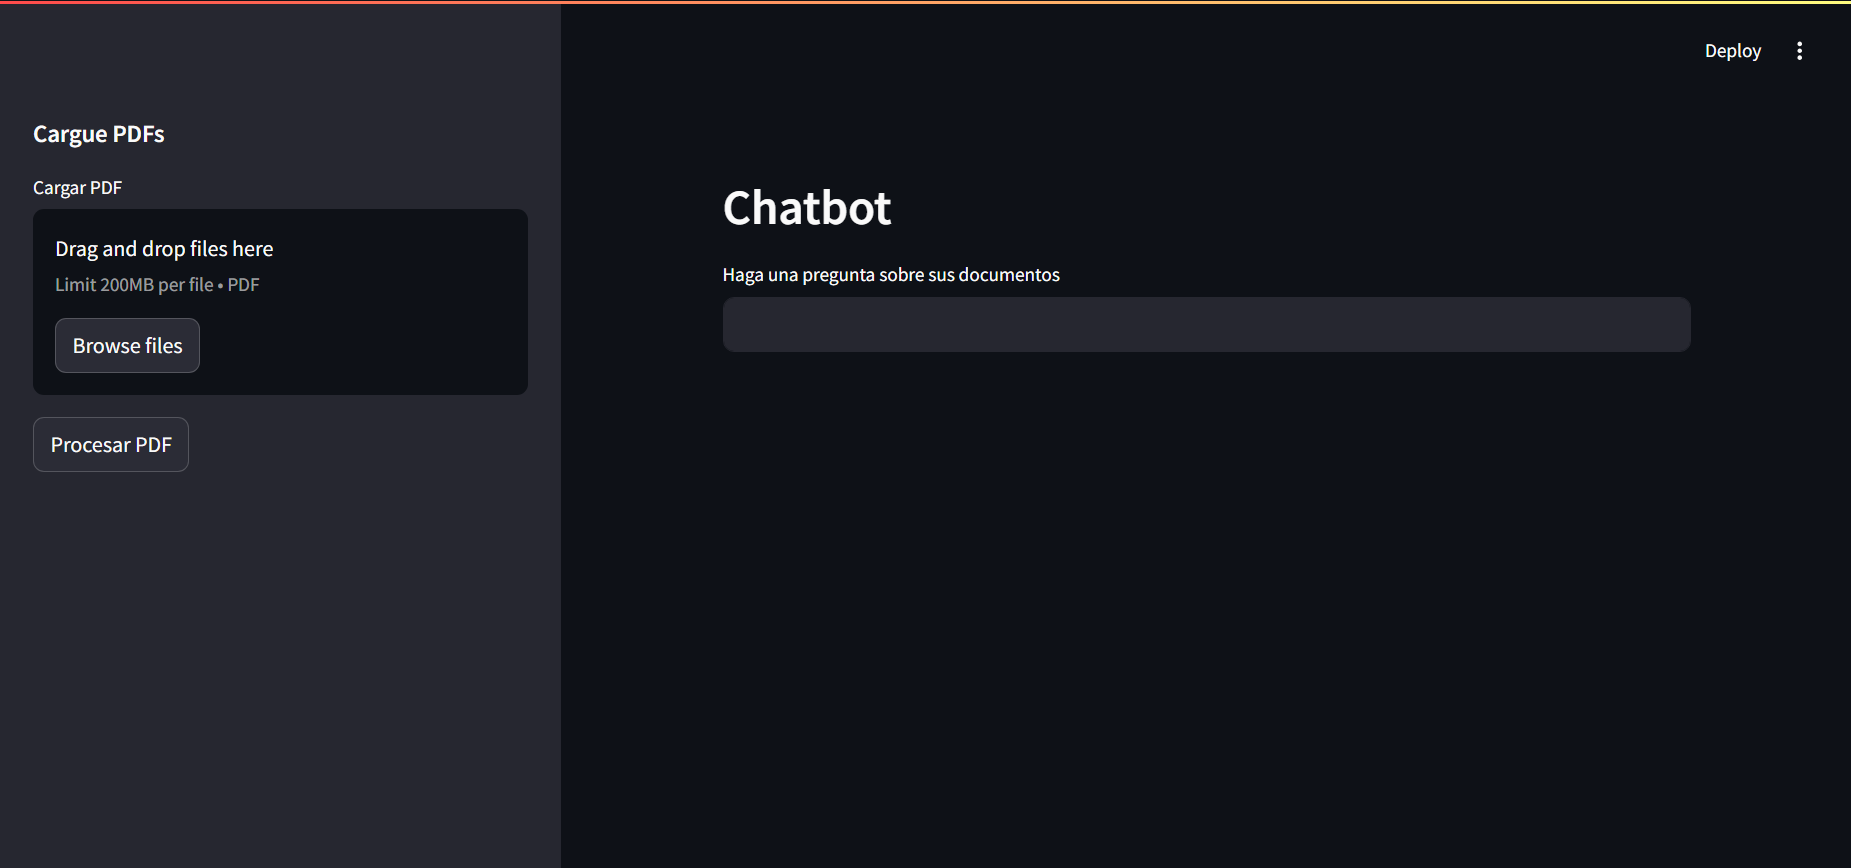
\includegraphics[width=1.0\linewidth]{chatbot.png}\end{figure}
\end{frame}
\note{
APÉNDICE: el sketch original (Streamlit) que sirvió de prueba de concepto.
Útil para mostrar la evolución del prototipo si preguntan.
}

\end{document}